\documentclass[twocolumn,10pt]{article}
\usepackage[margin=0.75in,columnsep=0.25in]{geometry}
\usepackage{booktabs}
\usepackage{graphicx}
\usepackage{amsmath}
\usepackage{microtype}
\usepackage[hidelinks]{hyperref}
\usepackage{xcolor}

\newcommand{\llmd}{llm-d}
\newcommand{\code}[1]{\texttt{\small #1}}

\title{\bf Peer-to-Peer KV-Cache Sharing for Distributed LLM Serving}
\author{
  Nili Guy \and Liran Schour \and (author list TBD)\\[2pt]
  \normalsize IBM Research
}
\date{Draft --- \today}

\begin{document}
\maketitle

\begin{abstract}
Prefix KV caches in distributed LLM serving are per-instance resources:
a prefix cached on one pod is recomputed on every other pod that serves
it. We describe a peer-to-peer (P2P) KV-cache sharing mechanism for the
\llmd{} inference stack in which any vLLM instance can pull cached
prefix blocks from a peer's CPU offload tier over the network, under a
router-side policy that requests a pull only when the expected saving
exceeds a calibrated threshold. The mechanism generalizes the
prefill/decode (P/D) disaggregation transfer path into a symmetric peer
protocol and composes with prefix-affinity routing, KV offloading, and
P/D disaggregation. We evaluate on three models and four workload
families on H200 clusters. A single-request analysis shows the pull
outperforming recomputation above a model-dependent crossover of
300--900 tokens, with the advantage growing with prefix length ($-68\%$
latency at 48K tokens). End to end, the mechanism pays in both
deployment modes. In aggregated serving, load-aware placement with the
pull cuts document-Q\&A tail TTFT by 28--74\% (up to $3.9\times$)
against prefix-affinity routing with up to $+17\%$ throughput, and
makes load-balanced placement viable for oversubscribed prefix pools.
Added to the \llmd{} P/D reference deployment, it is strictly
beneficial at high load: median TTFT drops $10.3\times$ with $+40\%$
throughput on document Q\&A, and $4.8\times$ with $+33\%$ throughput
on agentic session shapes (10--100K-token contexts, tool-call idle
gaps), while tail latency is bounded in both arms by the irreducible
cold prefill. We further show that placement policy, not
transfer capability, determines whether sharing pays: making the pull
the primary data path (load-only placement) scatters cache mass and
loses to prefix affinity at every load tested, whereas affinity
placement with pull-on-divergence wins consistently.
\end{abstract}

\section{Introduction}
Reuse of prefix KV state is one of the highest-leverage optimizations
in LLM serving: shared system prompts, common documents, multi-turn
histories, and agentic loops all re-present token prefixes whose
attention state has already been computed somewhere in the fleet.
Modern routers exploit this locally --- prefix-affinity routing steers a
request to the pod most likely to hold its prefix --- but affinity has
structural limits: sessions migrate under load balancing, replicas come
up cold on scale-out, and under contention the pod that owns a popular
prefix becomes the queueing bottleneck.

This paper describes and evaluates a complementary mechanism in the
\llmd{} stack: \emph{peer-to-peer KV-cache sharing}, in which the
missing prefix is transferred from the peer that holds it instead of
recomputed. Three design decisions distinguish the system:
(i)~transfers are served from the CPU offload tier, off the GPU and off
the request's failure path (a failed or partial pull degrades to
recomputation); (ii)~the pull decision is made centrally by the
router's endpoint picker (EPP), reusing the same per-pod prefix-cache
index that powers affinity routing; and (iii)~the decision is gated by
a per-model calibrated threshold so a pull is requested only when the
peer's cached advantage exceeds the transfer's break-even point.

We report a measurement-driven evaluation: a single-request
pull-versus-recompute analysis that prices the mechanism per model
(\S\ref{sec:crossover}); fleet-level results in aggregated serving
(\S\ref{sec:agg}); paired end-to-end comparisons on the \llmd{}
P/D reference topology under document-Q\&A and agentic workloads
(\S\ref{sec:e2e}); a mechanism study showing router-decided
prefill$\leftarrow$decode transfers sustaining flat per-turn latency in
multi-turn chat (\S\ref{sec:mech}); and a negative result
(\S\ref{sec:placement}): using the pull as the primary placement
strategy loses to prefix affinity at every load we tested, on two
independent implementations.

\section{Background and Design}
\label{sec:design}
\paragraph{Setting.} \llmd{} deploys vLLM instances behind an inference
gateway. An endpoint-picker (EPP) scores candidate pods per request;
prefix-cache scorers use either an approximate index (routing history)
or a precise index fed by engine KV events. vLLM's offloading connector
spills KV blocks from GPU HBM to a CPU memory tier; P/D disaggregation
runs separate prefill and decode workers connected by NIXL.

\paragraph{Mechanism.} The P2P connector generalizes the P/D transfer
path into a symmetric peer protocol. Every instance can act as
\emph{producer} (serving blocks from its CPU tier) and \emph{consumer}
(pulling blocks it lacks). A consumer sends the block hashes it needs
over a ZMQ control channel; the producer answers with its hits; NIXL
moves the matched blocks CPU-tier to CPU-tier; hits then load into the
consumer's GPU as ordinary cache hits and misses are recomputed.
Transfers are asynchronous and best-effort.

\paragraph{Policy.} The EPP compares, for each request, the
best-cached candidate against the pod that will compute the prefix
(under P/D, the prefill worker). When the peer's cached-token advantage
exceeds \code{minCachedTokenDelta}, the EPP attaches a source header;
the routing sidecar translates it into connector transfer parameters on
the prefill leg. Ties and self-matches never trigger a pull.

\paragraph{Deployment invariants.} Block hashes must agree fleet-wide
(identical \code{--block-size} and hash seed), peers must run the same
tensor-parallel degree (KV block identity is TP-dependent), and the CPU
tier should be provisioned at roughly $2\times$ the \emph{measured} GPU
KV capacity, since its value is the KV that the GPU evicts and the CPU
retains.

\section{Single-Request Economics}
\label{sec:crossover}
Figure~\ref{fig:crossover} prices the mechanism on gpt-oss-120b (one
H200 per pod): prefill latency for a fully cached prefix, recomputed
locally versus pulled from a peer's CPU tier (5-repetition medians).
The pull wins at every measured length and the gap widens with size,
reaching $-68\%$ at 48K tokens (551\,ms versus 1{,}695\,ms). On
Llama-3.1-8B the curves cross near 2K tokens; on gpt-oss the pull
already wins at 2K because its KV footprint per token is small relative
to its prefill speed. A two-point field procedure (time one warm pull
and one fresh recompute at a small and a large size) recovers the fixed
transfer overhead ($\approx$30\,ms) and both per-token rates, and hence
the crossover, in minutes on a live pod pair; on Qwen3-30B-A3B it
yields $\approx$760 tokens, and the deployments below set the threshold
one power of two above their measured crossover
(Table~\ref{tab:calib}).

\begin{figure}[t]
  \centering
  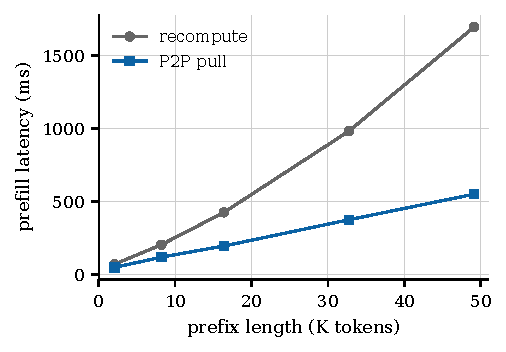
\includegraphics[width=\linewidth]{figures/crossover.pdf}
  \caption{Prefill latency for a fully cached prefix: local recompute
  versus P2P pull from a peer CPU tier. gpt-oss-120b, single
  source--consumer pair, 5-rep medians.}
  \label{fig:crossover}
\end{figure}

\begin{table}[t]
  \centering\small
  \caption{Measured pull-versus-recompute crossover and the deployed
  pull threshold.}
  \label{tab:calib}
  \begin{tabular}{lrr}
    \toprule
    model & crossover (tokens) & threshold \\
    \midrule
    gpt-oss-120b & $<2\,048$ & 2\,048 \\
    Llama-3.1-8B & $\approx 2\,000$ & 2\,048 \\
    Qwen3-30B-A3B & $\approx 760$ & 1\,024 \\
    \bottomrule
  \end{tabular}
\end{table}

\section{Fleet-Level Results: Aggregated Serving}
\label{sec:agg}
In aggregated serving every pod is a symmetric peer. We evaluate on
14$\times$gpt-oss-120b (one H200 each, 88\,GiB CPU tier per pod) with
the precise prefix index, and replicate mechanisms on
4$\times$Llama-3.1-8B.

\paragraph{Document Q\&A.} 192 distinct $\approx$49K-token documents,
6 questions each, 128 conversations in flight --- a working set that
oversubscribes the fleet's GPU caches, so placement decides between a
cache hit, a recompute, and a queue. Two arms --- precise
prefix-affinity routing versus load-aware placement with the pull ---
with arm order alternated across two full runs (all four runs
1{,}152/1{,}152, zero failures). Medians are equal: a session answering
from its warm cache is fast either way. The arms separate on tails and
stability: p99 TTFT 21--27\,s with the pull versus 37--81\,s under
affinity --- a 28--74\% reduction, up to $3.9\times$ --- alongside up to
$+17\%$ throughput and a 10\% run-to-run spread versus 28\%.
Affinity concentrates each document's questions on its owner, whose
queue becomes the p99 while displaced questions recompute 49K tokens;
load-aware placement sends questions wherever capacity exists, and the
pull prices the resulting miss at $\approx$0.6\,s instead of a
$\approx$2\,s recompute or a multi-second wait. The P2P arm moved
30--32M tokens between pods per run.

\paragraph{Hot prefix and prefix pools.} With a single hot 16K prefix,
load-balanced routing alone wins ($11\times$ lower median latency than
affinity's owner-saturation at 24\,req/s); the pull adds nothing once
the prefix is resident everywhere --- its role is to make load-balanced
routing safe when prefixes do \emph{not} fit everywhere. A 64-prefix
pool (128\,GiB of KV, far exceeding any pod's cache) measures exactly
that: every off-owner arrival either recomputes 16K tokens or pulls
them, and the pulled arm sustains rates the recompute arm cannot
(saturating $\approx$10.4 versus 12.6\,req/s at the highest tested
offered rate, with p50 latency an order of magnitude lower under
overload).

\section{End-to-End Results on the P/D Reference Topology}
\label{sec:e2e}
We compare the \llmd{} P/D reference deployment exactly as shipped
(arm~A) against the identical deployment plus the P2P stack --- CPU
offload tier and pull --- with placement policy unchanged (arm~B). Each
arm runs on a freshly provisioned fleet; workloads and arms complete
all requests with zero failures.

\paragraph{Document Q\&A.} gpt-oss-120b on 16$\times$H200 (8 prefill +
8 decode, TP=1); 192 conversations $\times$ 6 turns over
$\approx$49K-token documents at concurrency 192
(Table~\ref{tab:paired}, left; Figure~\ref{fig:paired}). Median TTFT
improves $10.3\times$ and throughput $+40\%$. The dominant effect at
this operating point is the offload tier serving history re-prefills
(52M externally served tokens) that arm~A recomputes under 192-deep
queues.

\paragraph{Agentic sessions.} Qwen3-30B-A3B-Thinking on 6$\times$H200
(2 prefill + 4 decode, TP=1), the agentic-serving reference shapes:
10--100K-token contexts, 4--40 turns, tool-call gaps of 1--20\,s that
evict session KV between turns; 288 requests at concurrency 16
(Table~\ref{tab:paired}, right). Median TTFT improves $4.8\times$ with
$+33\%$ throughput, and 1.23M tokens of session history are pulled
instead of recomputed in a 229\,s run (a second arm-B sample reproduces
the result: p50 1.06\,s, 237\,s). The p99 is unchanged by construction:
both arms' worst case is the cold first prefill of a 100K-token
context; the pull removes re-computation, not first computation.

\begin{table}[t]
  \centering\small
  \caption{Paired end-to-end results on the P/D reference topology.
  All arms complete all requests (1{,}152 and 288 respectively) with
  zero failures.}
  \label{tab:paired}
  \begin{tabular}{lrr@{\hspace{1.2em}}rr}
    \toprule
    & \multicolumn{2}{c}{document Q\&A} & \multicolumn{2}{c}{agentic} \\
    \cmidrule(r){2-3}\cmidrule(l){4-5}
    metric & guide & +P2P & guide & +P2P \\
    \midrule
    TTFT p50 (s) & 11.94 & \textbf{1.16} & 5.22 & \textbf{1.09} \\
    TTFT p95 (s) & 71.6 & \textbf{55.2} & 18.94 & \textbf{11.77} \\
    TTFT p99 (s) & 106.1 & \textbf{80.0} & 30.29 & 29.98 \\
    throughput & 5.68/s & \textbf{7.96/s} & 288/304s & \textbf{288/229s} \\
    \bottomrule
  \end{tabular}
\end{table}

\begin{figure*}[t]
  \centering
  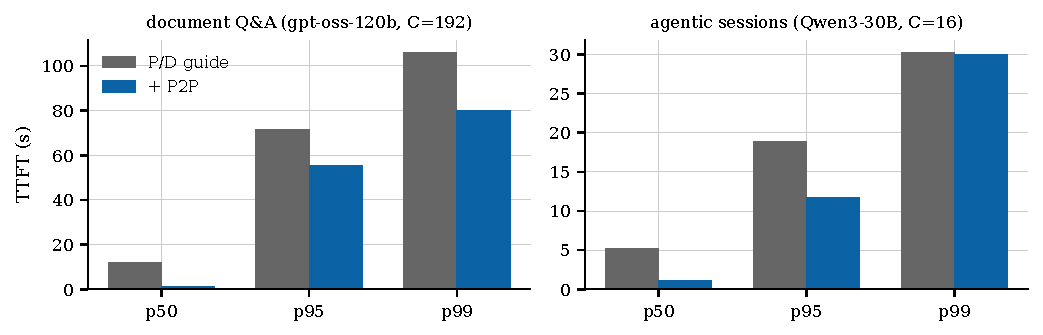
\includegraphics[width=0.85\textwidth]{figures/paired.pdf}
  \caption{TTFT percentiles for the paired arms of
  Table~\ref{tab:paired}.}
  \label{fig:paired}
\end{figure*}

\section{Mechanism: Router-Decided Prefill$\leftarrow$Decode Pulls}
\label{sec:mech}
Under P/D disaggregation the newest KV of a conversation lives on the
decode worker: it received the prompt over NIXL and generated the
answer. On the next turn, the scheduled prefill worker lacks that
history; the EPP's precise index --- fed by KV events from both roles ---
observes the decoder's advantage and requests the pull. We measure this
on Llama-3.1-8B chat multi-turn (4 prefill + 4 decode, 48 conversations
$\times$ 8 turns, live message history): 477K tokens of session history
move decoder$\to$prefiller in one run, and per-turn TTFT holds at
0.1--0.2\,s while prompts grow from 5K to 20K tokens
(Figure~\ref{fig:turns}). On a model this small the replaced recompute
is also cheap, so the benefit is prefill capacity rather than visible
latency; the latency benefit scales with history size and prefill cost,
which is what \S\ref{sec:e2e}'s agentic result realizes.

\begin{figure}[t]
  \centering
  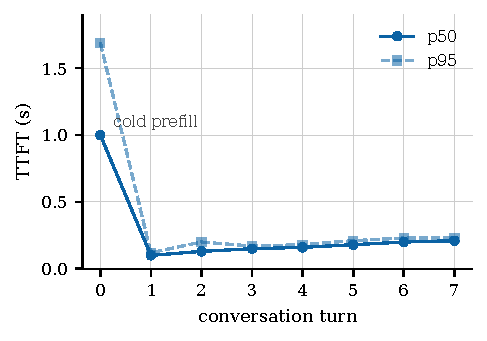
\includegraphics[width=\linewidth]{figures/turns.pdf}
  \caption{Per-turn TTFT with router-decided
  prefill$\leftarrow$decode pulls (Llama-3.1-8B, 48 conversations
  $\times$ 8 turns). Turn 0 pays the cold prefill; later turns' history
  arrives by pull as prompts grow 5K$\to$20K tokens.}
  \label{fig:turns}
\end{figure}

\section{Placement Policy Dominates Transfer Capability}
\label{sec:placement}
A natural alternative design treats the pull as the primary data path:
place requests purely by load and pull the prefix wherever it lands. We
tested this on two independent implementations --- our own load-first
arm on the document-Q\&A workload, and an independent
wide-expert-parallel deployment at data-parallel degree 16 --- and it
loses to prefix affinity at every load tested, with the deficit
\emph{growing} with concurrency. The failure is structural. Affinity
compounds: a pod that serves turn $N$ serves turn $N{+}1$ from local
cache, and its cache mass grows. Load-only placement scatters arrivals,
so cache mass never accumulates and the best peer's coverage per
request shrinks as concurrency rises (recomputation share rising from
24.8\% to 28.7\% across the tested ladder in the independent
deployment). Pulled copies also churn the destination tiers, evicting
locally accumulated KV (local hit rate falling to 17\%), and sustained
transfer bandwidth saturates ($\approx$4.2\,GB/s observed) while
affinity's hits consume none. The winning configuration in every
experiment keeps affinity placement and uses the pull as the recovery
path for genuine divergence --- queue-pressure spills, evictions across
idle gaps, cold replicas, migrations --- which is also the configuration
whose pull volumes are millions of tokens per run rather than
terabytes.

\section{Limitations}
\label{sec:limits}
Pulling a \emph{generated} turn requires the follow-up request to
reproduce the generated token IDs. Chat-templated APIs achieve this for
models whose templates re-render assistant turns verbatim (our
Llama-3.1-8B measurement); models that drop reasoning segments on
re-render (gpt-oss, Qwen3-Thinking) expose only input context and
re-prefilled history for pulling --- in the agentic workloads measured
here, the bulk of the reuse. Text-append clients (as in common
benchmark harnesses) cannot exercise generated-turn reuse for any
model, because re-tokenized text diverges from generated IDs. KV block
identity is tensor-parallel-dependent in the connector, so peers must
run matched TP; and per-peer sessions are established lazily, so the
first contact between a pair proceeds as a recompute unless sessions
are pre-established.

\section{Conclusion}
P2P KV-cache sharing converts \llmd{}'s per-pod prefix caches into a
fleet resource under a router-owned, threshold-gated policy. Measured
on H200 clusters across three models, it is strictly beneficial as an
addition to the P/D reference deployment --- $10.3\times$ and
$4.8\times$ median TTFT on document-Q\&A and agentic workloads with
$+40\%$ and $+33\%$ throughput --- provided it is deployed as a recovery
path under affinity placement, with the threshold set from a measured
per-model crossover.

\end{document}
